\section{非齐次方程}
\label{sec:lde-inhomogeneous}

齐次传播建立之后，再加入外部输入。设$\bm{A}$、$\bm{g}$在区间$I$上连续，考虑
\begin{equation}
 \dot{\bm{x}}(t)=\bm{A}(t)\bm{x}(t)+\bm{g}(t),\qquad \bm{x}(t_0)=\bm{x}_0.
 \label{eq:lde-inhomogeneous}
\end{equation}
输入在每一时刻都推动状态，推动的效果又随齐次系统继续传播。怎样把这两件事合写成一个公式？

\paragraph{常数变易}
没有输入时，解是$\bm{\Phi}(t,t_0)\bm{c}$，其中$\bm{c}$是常向量，等于初始状态。输入不断改变状态，可以理解为“初始状态”这个系数在缓慢漂移。于是让$\bm{c}$依赖时间，设$\bm{x}(t)=\bm{\Phi}(t,t_0)\bm{c}(t)$，代入方程。

乘积求导时，$\partial_t\bm{\Phi}$产生的项恰好是$\bm{A}\bm{x}$，与方程右端抵消，只剩下
\[
 \bm{\Phi}(t,t_0)\dot{\bm{c}}(t)=\bm{g}(t).
\]
用$\bm{\Phi}(t,t_0)^{-1}=\bm{\Phi}(t_0,t)$乘两边，再由$\bm{c}(t_0)=\bm{x}_0$积分，得到
\[
 \bm{c}(t)=\bm{x}_0+\int_{t_0}^{t}\bm{\Phi}(t_0,s)\bm{g}(s)\,\mathrm{d}s.
\]

这一步也有含义：$\bm{\Phi}(t_0,s)\bm{g}(s)$把时刻$s$的输入折算回初始时刻。把$\bm{c}(t)$代回去，再用复合关系$\bm{\Phi}(t,t_0)\bm{\Phi}(t_0,s)=\bm{\Phi}(t,s)$，就得到下面的定理。

\begin{theorem}[常数变易公式]
\label{thm:lde-variation-of-constants}
设$\bm{A},\bm{g}$在$I$上连续，$t_0\in I$。初值问题~\eqref{eq:lde-inhomogeneous}在$I$上有唯一解，它是
\begin{equation}
 \bm{x}(t)=\bm{\Phi}(t,t_0)\bm{x}_0+\int_{t_0}^{t}\bm{\Phi}(t,s)\bm{g}(s)\,\mathrm{d}s.
 \label{eq:lde-variation-of-constants}
\end{equation}
常系数时$\bm{\Phi}(t,s)=\mathrm{e}^{(t-s)\bm{A}}$，公式成为
\begin{equation}
 \bm{x}(t)=\mathrm{e}^{(t-t_0)\bm{A}}\bm{x}_0+\int_{t_0}^{t}\mathrm{e}^{(t-s)\bm{A}}\bm{g}(s)\,\mathrm{d}s.
 \label{eq:lde-duhamel-constant}
\end{equation}
\end{theorem}

\begin{proof}
先检验式~\eqref{eq:lde-variation-of-constants}满足方程和初值。由复合关系，这个公式可以写成乘积$\bm{\Phi}(t,t_0)\bm{c}(t)$，其中$\bm{c}$如上。对乘积求导，得
\[
\begin{aligned}
 \dot{\bm{x}}(t)&=\bm{A}(t)\bm{\Phi}(t,t_0)\bm{c}(t)+\bm{\Phi}(t,t_0)\bm{\Phi}(t_0,t)\bm{g}(t)\\
 &=\bm{A}(t)\bm{x}(t)+\bm{g}(t).
\end{aligned}
\]
$t=t_0$时积分为零，$\bm{\Phi}(t_0,t_0)=\bm{I}$，所以$\bm{x}(t_0)=\bm{x}_0$。

再证唯一。两个解之差满足齐次方程，初值为零，由定理~\ref{thm:lde-transition-existence}恒为零。
\end{proof}

式~\eqref{eq:lde-variation-of-constants}称为\term{常数变易公式}（variation of constants formula），也称\term{Duhamel公式}（Duhamel formula）。若$\bm{g}$只在每个紧子区间上可积，公式不变，解是局部绝对连续的，方程几乎处处成立，这与定理~\ref{thm:lde-scalar-integrable}的论证相同。

\paragraph{初始状态响应与零初值响应}
公式的两项分别只含一种数据。第一项$\bm{\Phi}(t,t_0)\bm{x}_0$不依赖输入，称为\term{零输入响应}（zero-input response）。第二项不依赖初始状态，称为\term{零状态响应}（zero-state response）。

每一项都线性依赖自己的数据，总响应是两项之和。所以“响应”对数据对$(\bm{x}_0,\bm{g})$是线性的。常见的误解是说总响应关于输入线性：若$\bm{x}_0\neq\bm{0}$，把输入加倍并不会把总响应加倍，因为零输入响应没有变。

\begin{example}[阶跃输入的响应分解]
\label{ex:lde-step-response}
考虑$\ddot{x}+3\dot{x}+2x=1$，$x(0)=1$，$\dot{x}(0)=0$。状态形式用例~\ref{ex:lde-running-system}的矩阵，$\bm{g}=(0,1)^{\top}$，$\bm{x}_0=(1,0)^{\top}$。零输入响应的第一分量已经算过，是$2\mathrm{e}^{-t}-\mathrm{e}^{-2t}$。

零状态响应用到$\mathrm{e}^{r\bm{A}}$的第二列，它的第一分量是$\mathrm{e}^{-r}-\mathrm{e}^{-2r}$。在式~\eqref{eq:lde-duhamel-constant}中令$r=t-s$，积分变成
\[
 \int_0^t(\mathrm{e}^{-r}-\mathrm{e}^{-2r})\,\mathrm{d}r=\frac12-\mathrm{e}^{-t}+\frac12\mathrm{e}^{-2t}.
\]
两部分相加，得到总响应
\[
 x(t)=\frac12+\mathrm{e}^{-t}-\frac12\mathrm{e}^{-2t}.
\]
代回检验：$x(0)=1$，$\dot{x}=-\mathrm{e}^{-t}+\mathrm{e}^{-2t}$，所以$\dot{x}(0)=0$；再求$\ddot{x}=\mathrm{e}^{-t}-2\mathrm{e}^{-2t}$，并计算
\[
 \ddot{x}+3\dot{x}+2x=(1-3+2)\mathrm{e}^{-t}+(-2+3-1)\mathrm{e}^{-2t}+1=1.
\]
\end{example}

图~\ref{fig:lde-response-decomposition}中，黄线由初始状态决定，从$1$下降到$0$；紫线由输入决定，从$0$升到$1/2$。蓝线是二者之和。这个系统的状态最终停在$1/2$，只和输入有关，初值的痕迹全部由零输入响应带走。

\begin{BookInlineFigure}
  \centering
  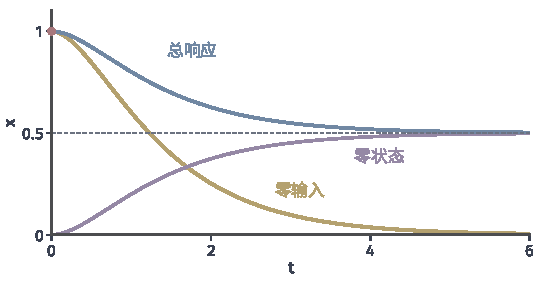
\includegraphics[width=92mm]{figures/06-differential-equations/01-ordinary-differential-equations/matplotlib/lde-response-decomposition/figure.pdf}
  \caption{响应的分解，方程$\ddot{x}+3\dot{x}+2x=1$，$x(0)=1$（红点），$\dot{x}(0)=0$。黄线是零输入响应，紫线是零状态响应，蓝线是总响应，灰色虚线是水平$1/2$。}
  \label{fig:lde-response-decomposition}
\end{BookInlineFigure}

\paragraph{受迫振动与共振}
荡秋千时，每次都在同一相位推一下，幅度就越来越大；推的节奏不对，推力再大也荡不高。把这个现象写成方程，就是无阻尼振子受周期外力：
\begin{equation}
 \ddot{x}+\omega_0^2x=\cos\omega t,\qquad x(0)=\dot{x}(0)=0,
 \label{eq:lde-forced-oscillator}
\end{equation}
其中$\omega_0>0$是固有频率，$\omega>0$是外力频率。

状态形式的系数矩阵如下，它满足$\bm{A}^2=-\omega_0^2\bm{I}$：
\[
 \bm{A}=\begin{bmatrix}0&1\\-\omega_0^2&0\end{bmatrix}.
\]
级数的偶次项和奇次项分别凑成余弦和正弦，得到
\[
 \mathrm{e}^{t\bm{A}}=\begin{bmatrix}\cos\omega_0t&\sin(\omega_0t)/\omega_0\\-\omega_0\sin\omega_0t&\cos\omega_0t\end{bmatrix}.
\]
输入是$(0,\cos\omega t)^{\top}$，所以式~\eqref{eq:lde-duhamel-constant}的第一分量是
\begin{equation}
 x(t)=\frac{1}{\omega_0}\int_0^t\sin\bigl(\omega_0(t-s)\bigr)\cos(\omega s)\,\mathrm{d}s.
 \label{eq:lde-forced-integral}
\end{equation}

用积化和差把被积函数拆开：
\[
 \begin{aligned}
 \sin(\omega_0(t-s))\cos\omega s={}&\tfrac12\sin\bigl(\omega_0t-(\omega_0-\omega)s\bigr)\\
 &+\tfrac12\sin\bigl(\omega_0t-(\omega_0+\omega)s\bigr).
 \end{aligned}
\]
当$\omega\neq\omega_0$时，两项都对$s$积分，第一项给出$(\cos\omega t-\cos\omega_0t)/(\omega_0-\omega)$，第二项给出$(\cos\omega t-\cos\omega_0t)/(\omega_0+\omega)$。代入式~\eqref{eq:lde-forced-integral}并通分，
\begin{equation}
 x(t)=\frac{\cos\omega t-\cos\omega_0t}{\omega_0^2-\omega^2},\qquad \omega\neq\omega_0.
 \label{eq:lde-off-resonance}
\end{equation}
这个解有界，幅度不超过$2/\lvert\omega_0^2-\omega^2\rvert$。$\omega$接近$\omega_0$时，两个余弦的频率相近，交替增强与抵消，形成缓慢起伏的\term{拍}（beat）。

当$\omega=\omega_0$时，第一项是常数$\tfrac12\sin\omega_0t$，它对$s$积分得到$\tfrac12t\sin\omega_0t$。第二项在$[0,t]$上的积分为
\[
 \frac12\Bigl[\frac{\cos(\omega_0t-2\omega_0s)}{2\omega_0}\Bigr]_{s=0}^{s=t}=0.
\]
于是
\begin{equation}
 x(t)=\frac{t\sin\omega_0t}{2\omega_0},\qquad \omega=\omega_0.
 \label{eq:lde-resonance}
\end{equation}
代回检验，取$\omega_0=1$，$x=\tfrac12t\sin t$。两次求导得到
\[
 \dot{x}=\frac{\sin t+t\cos t}{2},\qquad \ddot{x}=\cos t-\frac{t\sin t}{2}.
\]
所以$\ddot{x}+x=\cos t$，并且$x(0)=\dot{x}(0)=0$。

这种振幅按$t$线性增长的现象称为\term{共振}（resonance）。图~\ref{fig:lde-resonance}取$\omega_0=1$比较三种外力频率。外力大小完全相同，差别只在频率：$\omega=2$时响应很小，$\omega=1.2$时出现拍，$\omega=1$时振幅沿紫色虚线$\pm t/2$增长。

\begin{BookInlineFigure}
  \centering
  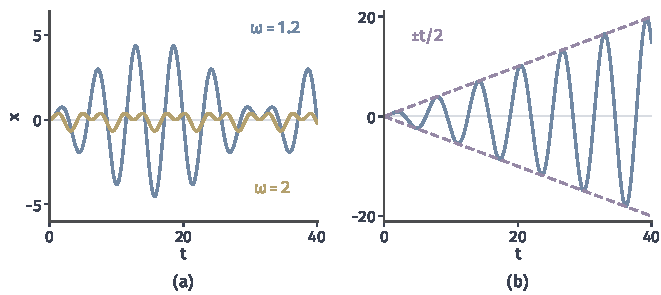
\includegraphics[width=112mm]{figures/06-differential-equations/01-ordinary-differential-equations/matplotlib/lde-resonance/figure.pdf}
  \caption{方程~\eqref{eq:lde-forced-oscillator}取$\omega_0=1$的零初值响应。(a)$\omega=2$（黄）的响应有界，$\omega=1.2$（蓝）出现拍。(b)$\omega=1$时发生共振，响应$t\sin t/2$的振幅沿紫色虚线$\pm t/2$线性增长。}
  \label{fig:lde-resonance}
\end{BookInlineFigure}

共振的原因要看积分~\eqref{eq:lde-forced-integral}的被积函数。$\sin(\omega_0(t-s))$是时刻$s$的单位冲击到时刻$t$还留下的响应，$\cos\omega s$是那一刻的外力。图~\ref{fig:lde-resonance-integrand}固定$t=4.5\pi$，画出被积函数对$s$的形状。

$\omega=1$时被积函数不变号，每一时刻的贡献都同向累加，面积是$t/2\approx7.07$。$\omega=2$时正负面积大部分抵消，只剩$1/3$。所以共振并不是输入太大，而是输入与齐次模式同频，各时刻留下的响应到达同一时刻时相位一致。

这与第~\ref{sec:lde-constant}节的多项式因子是同一个机制：Jordan链上一级的输出含有下一级自身的模式，这里外力含有振子自身的模式，于是都多出一个因子$t$。无阻尼模型的振幅没有上界。若有阻尼，齐次模式按指数衰减，早期输入留下的响应会逐渐消失，累积不再无限制地增长。

\begin{BookInlineFigure}
  \centering
  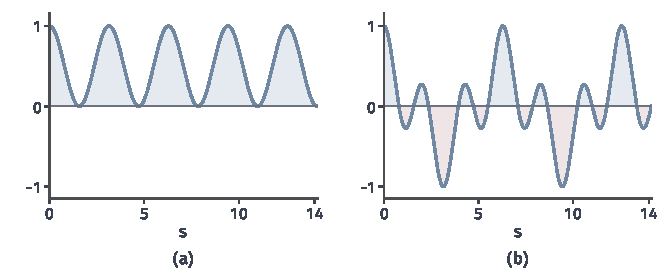
\includegraphics[width=112mm]{figures/06-differential-equations/01-ordinary-differential-equations/matplotlib/lde-resonance-integrand/figure.pdf}
  \caption{共振的累积机制。式~\eqref{eq:lde-forced-integral}取$\omega_0=1$、$t=4.5\pi$时的被积函数$\sin(t-s)\cos\omega s$，浅蓝为正面积，浅红为负面积。(a)$\omega=1$，被积函数不变号，积分约为$7.07$。(b)$\omega=2$，正负抵消，积分为$1/3$。}
  \label{fig:lde-resonance-integrand}
\end{BookInlineFigure}
